\documentclass[13pt,oneside]{book}
\usepackage[utf8]{inputenc}
\usepackage{url}
\usepackage{listings}
\usepackage{graphicx}

\usepackage{geometry}
\geometry{a4paper, left=20mm, right=20mm, top=20mm, bottom=20mm}
\usepackage[margin=1.2in]{geometry}
\usepackage[toc,page]{appendix}
\usepackage{graphicx}
\usepackage{natbib}
\usepackage{lipsum}
\usepackage{caption}

\begin{document}

\captionsetup[figure]{margin=1.5cm,font=small,labelfont={bf},name={Figure},labelsep=colon,textfont={it}}
\captionsetup[table]{margin=1.5cm,font=small,labelfont={bf},name={Table},labelsep=colon,textfont={it}}
\setlipsumdefault{1}

\begin{titlepage}
\begin{center}
{\LARGE College Of Engineering Trivandrum}\\[3cm]
\linespread{1.2}\huge {\bfseries System Software Lab}\\[3cm]
\linespread{1}

\includegraphics[width=5cm]{img/emblem.jpeg}\\[3cm]
{\Large GOKUL K\\ S5  CSE \\ Roll No:21\\ TVE18CS021 }\\[1cm]


\textit{ }\\[2cm]
Department of Computer Science\\[0.2cm]
\today
\end{center}

\end{titlepage}

\newpage

\begin{frame}{}
    \centering
    \hspace*{-0.5cm}
    $\vcenter{\hbox{
\includegraphics[width=1.5cm]{img/emblem.jpeg}}}$
    $\vcenter{\resizebox{0.95\textwidth}{!}{
        \begin{tabular}{c}
             CS331 - System Software Lab $\cdot$ 2020 $\cdot$   \\
             \hline 
        \end{tabular}
    }}$
\end{frame}
\section*{Cycle 1}
\section*{Expt 3}
\begin{center}
    \Large{Page Replacement Algorithms}
\end{center}FCFS
\section*{Aim}
\large
Simulate the following page replacement algorithms.\\
a) FIFO\\
b) LRU \\
c) LFU \\

\section*{Algorithm}
    \subsection*{FIFO}
    \begin{verbatim}
		1 Start traversing the pages .
		2 If set holds less pages than capacity .
		3 Insert page into the set one by one until
		4 the size of set reaches capacity or all
		5 page requests are processed .
		6 Simultaneously maintain the pages in the
		7 queue to perform FIFO .
		8 Increment page fault
		9 Else
		10 If current page is present in set , do nothing .
		11 Else
		12 Remove the first page from the queue
		13 as it was the first to be entered in
		14 the memory
		15 Replace the first page in the queue with
		16 the current page in the string .
		17 Store current page in the queue .
		18 Increment page faults .
		19 Return page faults .
    \end{verbatim}  
    \subsection*{LRU}
    \begin{verbatim}
        1 Start traversing the pages .
		2 If set holds less pages than capacity .
		3 Insert page into the set one by one until
		4 the size of set reaches capacity or all
		5 page requests are processed .
		6 Simultaneously maintain the recent occurred
		7 index of each page in a map called indexes .
		8 Increment page fault
		9 Else
		10 If current page is present in set , do nothing .
		11 Else
		12 Find the page in the set that was least
		13 recently used . We find it using index array .
		14 We basically need to replace the page with
		15 minimum index .
		16 Replace the found page with current page .
		17 Increment page faults .
		18 Update index of current page .
		19 Return page faults .
    \end{verbatim}
    \subsection*{LFU}
    \begin{verbatim}
        1 Start traversing the pages .
		2 If set holds less pages than capacity .
		3 Insert page into the set one by one until
		4 the size of set reaches capacity or all
		5 page requests are processed .
		6 Simultaneously maintain the recent occurred
		7 index of each page in a map called indexes .
		8 Increment page fault
		9 Else
		10 If current page is present in set , do nothing .
		11 Else
		12 Find the page in the set that was least
		13 frequently used . We find it using index array .
		14 We basically need to replace the page with
		15 minimum index .
		16 Replace the found page with current page .
		17 Increment page faults .
		18 Update index of current page .
		19 Return page faults .
    \end{verbatim}  
    
    \section*{Source Code}
    \Large\textbf{fifo}
\small

\begin{lstlisting}[language=C]
void fifo(int * frames, int * pages, size_t n_frames, size_t n_pages)
{
	size_t i, queue = 0;
	int n_faults = 0, n_hits = 0;

	for(i = 0; i < n_pages; i++)
	{
		printf("\nCurrent page: %d", pages[i]);

		if(! contains(frames, n_frames, pages[i]))
		{
			frames[queue] = pages[i];
			++n_faults;
			printf("\nFault");
			queue = (queue+1) % n_frames;
		}
		else
		{
			++n_hits;
			printf("\nHit");
		}
		
		printf("\nFrames: ");
		print_arr(frames, n_frames);
	}

	printf("\nNumber of pages faults: %d\n", n_faults);
}
    \end{lstlisting}
    
        \Large\textbf{lru}
\small

\begin{lstlisting}[language=C]
int find_lru(int * last_used, int n)
{
	int lru = 0, lru_count = 0;

	for(size_t i = 0; i < n; ++i)
	{
		if(last_used[i] < lru_count)
		{
			lru_count = last_used[i];
			lru = i;
		}
		++i;
	}

	return lru;
}

void lru(int * frames, int * pages, size_t n_frames, size_t n_pages)
{
	size_t i, index;
	int n_hits = 0, n_faults = 0;
	int * last_used = malloc(n_frames * sizeof(int));

	for(i = 0; i < n_frames; i++) last_used[i] = 0;

	for(i = 0; i < n_pages; i++)
	{
		printf("\nCurrent page: %d", pages[i]);

		if(!(index = contains(frames, n_frames, pages[i])))
		{
			if(i < n_frames) index = i;
			
			else {
				index = find_lru(last_used, n_frames);
			}

			++n_faults;
			printf("\nFault");
			frames[index] = pages[i];
		}
		else
		{
			++n_hits;
			printf("\nHit");
		}
		last_used[index] = n_faults + n_hits;
		printf("\nFrames: ");
		print_arr(frames, n_frames);
	}

	printf("\nNumber of faults: %d\n", n_faults);
}
    \end{lstlisting}
        \Large\textbf{lfu}
\small

\begin{lstlisting}[language=C]
int find_lfu(int * freq_used, int n)
{
	int lfu = 0, lfu_count = 0;

	for(size_t i = 0; i < n; ++i)
	{
		if(freq_used[i] < lfu_count)
		{
			lfu_count = freq_used[i];
			lfu = i;
		}
		++i;
	}

	return lfu;
}

void lfu(int * frames, int * pages, size_t n_frames, size_t n_pages)
{
	size_t i, index;
	int n_hits = 0, n_faults = 0;
	int * freq_used = malloc(n_frames * sizeof(int));

	for(i = 0; i < n_frames; i++) freq_used[i] = 0;

	for(i = 0; i < n_pages; i++)
	{
		printf("\nCurrent page: %d", pages[i]);

		if(!(index = contains(frames, n_frames, pages[i])))
		{
			if(i < n_frames) index = i;
			
			else {
				index = find_lfu(freq_used, n_frames);
			}

			++n_faults;
			printf("\nFault");
			frames[index] = pages[i];
		}
		else
		{
			++n_hits;
			printf("\nHit");
		}
		freq_used[index]++;
		printf("\nFrames: ");
		print_arr(frames, n_frames);
	}

	printf("\nNumber of faults: %d\n", n_faults);
}
	
    \end{lstlisting}
    \section*{Output}
    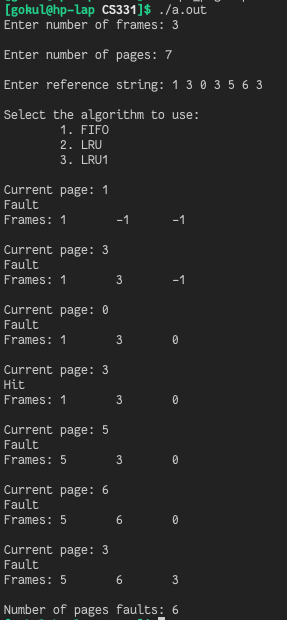
\includegraphics[]{img/p3/ss1.png} \\
    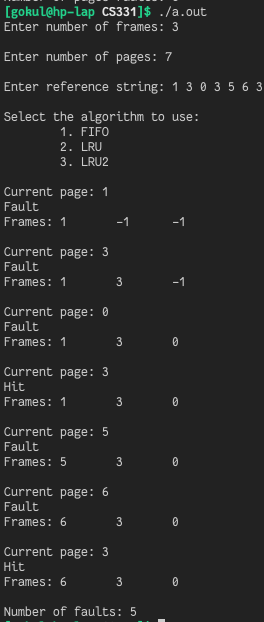
\includegraphics[]{img/p3/ss2.png} \\
    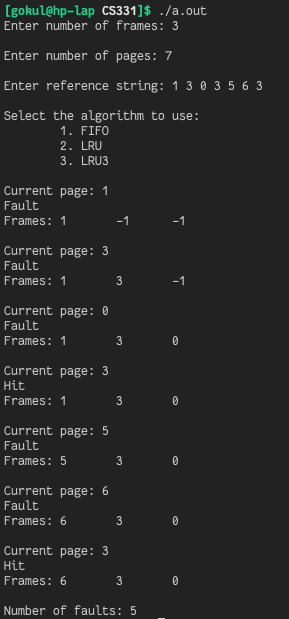
\includegraphics[]{img/p3/ss3.png} 
    
\Large
\section*{Result}
\large
The above algorithms were implemented and its output verified
\end{document}